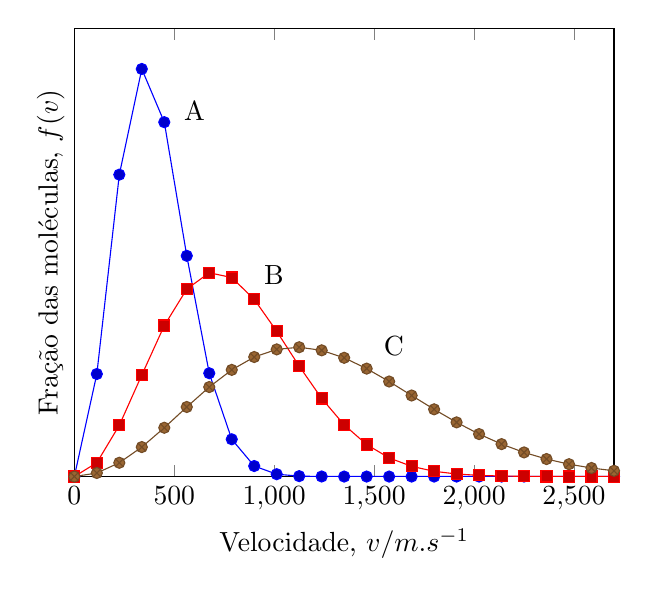
\begin{tikzpicture}
    \def\R{1000*8.314}% boltzmann constant
    \begin{axis}
        [
            grid = minor,
            domain = 0:2700,
            xlabel = {Velocidade, $v/\unit{m.s^{-1}}$},
            ylabel = {Fração das moléculas, $f(v)$},
            xmin=0, ymin=0,
            ytick = \empty,
            xmax=2700,
        ]
    \pgfplotsinvokeforeach{ 40, 10, 4 } % Ar, Ne, He
        {
            \addplot
                {
                    sqrt(2/pi)*(#1/(\R*298))^(3/2)*x^2*exp(-#1/(\R*298)*x^2/2)
                };
        }

    \node [anchor = south west] at (axis cs:500,0.002) 
        { \ce{A} };
    \node [anchor = south west] at (axis cs:900,0.00105) 
        { \ce{B} };
    \node [anchor = south west] at (axis cs:1500,0.00064) 
        { \ce{C} };
\end{axis}
\end{tikzpicture}

